\documentclass[11pt]{article}

\usepackage[letterpaper,margin=1in]{geometry}
\usepackage[T1]{fontenc}
\usepackage{amsmath,amsthm,mathtools}
\IfFileExists{newtxtext.sty}{\usepackage{newtxtext,newtxmath}}{\usepackage{mathptmx}\usepackage{amssymb}}
\usepackage{microtype}
\usepackage{setspace}
\usepackage{booktabs,tabularx,array}
\usepackage{enumitem}
\usepackage{xcolor}
\usepackage{tikz}
\usetikzlibrary{positioning}
\usepackage{natbib}
\usepackage[hidelinks]{hyperref}
\usepackage[nameinlink,noabbrev]{cleveref}

\definecolor{planner}{HTML}{2A78D6}
\definecolor{private}{HTML}{087D26}
\setstretch{1.035}
\setlength{\parskip}{0.25em}
\setlength{\parindent}{1.2em}
\setlength{\emergencystretch}{2em}
\Urlmuskip=0mu plus 1mu
\setlist{leftmargin=1.5em,itemsep=0.2em,topsep=0.3em}
\newtheorem{proposition}{Proposition}
\newtheorem{definition}{Definition}
\theoremstyle{remark}
\newtheorem{remark}{Remark}

\newcommand{\E}{\mathbb{E}}
\newcommand{\Prob}{\mathbb{P}}
\newcommand{\I}{\mathcal{I}}
\newcommand{\Pclass}{\mathcal{P}}
\newcommand{\RunID}{\texttt{20260720T190336Z\_DD-000\_32dd1c32\_217c602fa0}}

\title{\textbf{Foundations of Distributed Discovery}\\[0.35em]
\large Information, Action Allocation, and Incentives in Collective Search}
\author{Yohei Nakajima\\{\normalsize Untapped Capital}}
\date{July 2026}

\begin{document}
\maketitle

\begin{abstract}
Distributed discovery studies how groups convert dispersed evidence into portfolios of search actions. We define a discovery problem by its world, evidence process, information architecture, action technology, allocation protocol, budget, timing, reward rule, and discovery objective. For a declared feasible protocol class, the information frontier is the best discovery attainable from available evidence, while protocol loss is the value destroyed by an implemented action rule. This accounting separates better inference from better assignment. The Shared Discovery Paradox is the atomic one-period benchmark: pooling improves the highest-ranked candidate, but a one-answer protocol compresses a portfolio into a repeated choice. We connect that benchmark to team theory, information design, organizational search, coverage games, and adaptive/submodular search; distinguish redundancy from robustness; and organize open work on private-information teams, strategic disclosure, correlated sources, sequential feedback, overlapping coverage, mechanisms, and empirical audits. The note is a framework and research program, not a claim that the phrase or the surrounding literatures are new.
\end{abstract}

\noindent\textbf{Keywords:} distributed discovery, collective search, information architecture, action allocation, protocol loss, organizational search.\\
\textbf{Evidence note:} Claim identifiers in source comments refer to the repository ledger. Restated canonical results are attributed to \citet{Nakajima2026SharedDiscovery}; evidence status remains metric-specific.

\section{Introduction}
% Claims: DD-C-0001, DD-C-0017
Many collective-intelligence systems are evaluated as if they solve one problem: form the best belief and act on it. Discovery systems solve two. They must use evidence to rank candidates, and they must distribute finite action capacity over the candidate space. A committee can improve its estimate and still run a worse search if a one-answer convention makes every participant test the same hypothesis. Conversely, a coordinator can obtain coverage from weak information by assigning distinct actions. The first margin is informational; the second is allocative.

We use \emph{distributed discovery} as a working label for the design and analysis of systems that convert dispersed evidence into a finite portfolio of search actions. This definition is narrower than generic service or resource discovery and does not assert ownership of the phrase. The same wording appears in other technical settings, including autonomous-science agents \citep{WangEtAl2026DistributedDiscovery}. The project-specific object is the information--action separation, not a claim that collective search, decentralized teams, or epistemic diversity began here.

The motivating benchmark is the Shared Discovery Paradox \citep{Nakajima2026SharedDiscovery}. In its atomic environment, a target occupies one of many locations and each searcher receives a noisy private clue. Pooling the clues improves the best single recommendation. If all agents repeat that recommendation, however, group discovery can fall below independent clue-following. A planner using the same pooled reports can instead choose the highest-posterior portfolio and outperform both. The canonical paper develops that result, its strategic market benchmark, reward implementation, dependence extension, and scaling results. This note does not reproduce those proofs or replace its compact narrative. It asks what vocabulary survives after the atomic assumptions are relaxed.

The intellectual lineage is broad. Blackwell comparison orders information experiments for decision problems \citep{Blackwell1953}; team theory treats common-payoff agents with dispersed information \citep{MarschakRadner1972}; information design studies chosen disclosure \citep{KamenicaGentzkow2011}; and informational Braess effects show that more information can worsen equilibrium performance in another strategic technology \citep{AcemogluEtAl2018}. Organizational learning and the division of cognitive labor examine exploration, imitation, and heterogeneous research effort \citep{March1991,Kitcher1990,Zollman2007}. Coverage games, submodular maximization, adaptive search, and robot coverage supply neighboring allocation and robustness results \citep{Vetta2002,Gairing2009,NemhauserEtAl1978,GolovinKrause2011,HazonKaminka2008}. Scientific experiment choice provides a direct, richer application \citep{RzhetskyEtAl2015}.

Our contribution is organizational. We specify a common object; define information frontiers, protocol loss, recovery budgets, and evidence-aware diagnostics; separate information from assignment in an institutional matrix; and register which extensions require new results. The decomposition below is definitional. Its value lies in preventing a change in information, authority, incentives, or coverage technology from being mislabeled as the effect of another margin.

\subsection*{Evidence discipline}
The framework is paired with an evidence taxonomy because a research program can accumulate false certainty through presentation alone. A value emitted by a pinned script is not thereby an independent reproduction; a pattern over a finite grid is not a theorem; an identity defined by subtraction is not a substantive performance guarantee; and a plausible application mapping is not empirical evidence. These differences are recorded per claim rather than per paper. One document may contain a derived identity, independently reproduced finite values, sourced upstream theorems, exploratory observations, and unresolved questions.

The operational unit is a claim record linked to a proof, implementation, run, source, and tests where applicable. A computational run records its configuration, code and dependency versions, random seeds or explicit absence of randomness, outputs, checksums, and validation status. Failures remain visible but do not support substantive claims. This structure is more conservative than a single ``reproducible'' label and helps collaborators determine which result needs proof review, independent implementation, more computation, or external evidence.

The same discipline governs language. ``Exact'' refers to symbolic derivation or exhaustive finite evaluation with a stated arithmetic basis, not merely many printed digits. ``Verified'' means the declared check passed; it does not imply independence. ``Upstream result'' preserves the canonical source's scope. ``Open question'' is not upgraded because a heuristic found a good policy. This note uses those labels to complement the mathematics, not to substitute metadata for reasoning.

\section{Discovery architectures}
% Claims: DD-C-0001
\begin{definition}[Distributed discovery problem]
A distributed discovery problem is a tuple
\[
\mathcal D=(\Omega,\mu,E,I,A,\Gamma,B,\tau,R,v).
\]
Here $\Omega$ is the world space with prior $\mu$; $E$ is the evidence-generating kernel, including dependence and provenance; $I$ specifies information access; $A=\prod_i A_i$ is the joint action space; $\Gamma$ maps worlds and actions into covered outcomes; $B$ is the resource budget; $\tau$ describes timing, feedback, and stopping; $R$ gives private rewards or credit; and $v$ is the social discovery value.
\end{definition}

This tuple is deliberately redundant enough to expose modeling choices. A ``search action'' might open one box, run a wet-lab experiment, fund a prototype, query a database, or ask an agent to investigate a hypothesis. Its cost may be scalar, vector-valued, or state-dependent. Coverage may be modular, overlapping, stochastic, sequential, or valuable only in combination. The reward rule can differ from the social discovery objective, which is essential when autonomous agents choose strategically.

An information architecture describes which evidence, messages, and histories each decision maker can use. An action protocol is a stochastic kernel from those information histories into feasible joint actions. It covers centralized assignment, ex-ante role policies, independent local rules, equilibrium behavior, and adaptive policies, provided their feasibility and information are declared. A \emph{discovery architecture} is the implemented combination of information, protocol, and reward rule, holding the physical problem fixed.

This separation avoids three common ambiguities. First, ``decentralized'' can mean private information, autonomous action, or both. Second, ``more information'' can change equilibrium strategy as well as feasible inference. Third, repeated action can be waste, robustness, replication, or a necessary response to noisy execution. The tuple forces each interpretation into a primitive rather than leaving it in prose.

\subsection*{Feasibility is part of the object}
A protocol class must say who chooses mappings and when. A central planner choosing actions after observing all signals, a team committing to role policies before signals, and autonomous agents playing an equilibrium are different feasible sets even if their physical actions coincide. Shared randomness, public recommendations, private randomization, cheap talk, and binding assignments can each enlarge or reshape the set. Describing all of them as ``coordination'' erases the very margin the framework is meant to measure.

Timing matters equally. In a simultaneous design, every action is chosen before outcomes are known. A sequential design can condition later actions on failures, partial rewards, or revealed coverage. A parallel batch followed by adaptation lies between them. The budget may constrain total actions, concurrent actions, expected cost, worst-case cost, or stopping time. Two protocols with the same nominal count can therefore be incomparable until their timing and cost accounting are aligned.

Institutional authority is not always monotone in a behavioral model. Giving an organization a formal coordinator expands the set of assignable portfolios only if agents comply and the coordinator can use the relevant information. If the coordinator changes reporting incentives, crowds out local initiative, or selects a different objective, the physical feasible set and implemented outcome move together. Frontier monotonicity applies to set inclusion or emulation; claims about realized organizations require an implementation model.

Finally, the social objective $v$ must be separated from private rewards $R$. Discovery may value at least one success, the number or diversity of successful outcomes, information gained, time to first success, robustness, or downstream payoff. Credit may be equal-split, winner-take-all, marginal contribution, rank-based, or unrelated to coverage. Without both objects, ``incentive loss'' is indistinguishable from disagreement about what counts as discovery.

For a protocol $\Pi$, let $S_\Pi$ denote the induced action set, multiset, or sequence. Expected discovery under budget $B$ and architecture $I$ is
\[
G_B(\Pi;I)=\E_{\omega,E,\Pi}\left[v_\omega(S_\Pi)\right].
\]
Every expectation here depends on the declared evidence kernel, protocol randomization, and any execution noise. The notation suppresses these only after they are fixed.

\section{Information frontiers and protocol loss}
% Claims: DD-C-0002, DD-C-0016
Let $\Pclass_B(I)$ be the feasible protocol class given information $I$, budget $B$, action technology, timing, and institutional authority. Define
\[
V_B(I)=\sup_{\Pi\in\Pclass_B(I)}G_B(\Pi;I),
\qquad
L_B(\Pi;I)=V_B(I)-G_B(\Pi;I).
\]
The resulting Information--Action Decomposition is the identity
\begin{equation}
\boxed{G_B(\Pi;I)=V_B(I)-L_B(\Pi;I).}
\label{eq:decomposition}
\end{equation}
It is not an efficiency theorem. Changing the feasible protocol class changes the frontier; changing the benchmark changes the loss. A reported protocol-loss number is therefore incomplete without the information architecture, budget, authority, timing, objective, and action technology.

\begin{proposition}[Frontier monotonicity under emulation]
If every protocol in $\Pclass_B(I_1)$ can be emulated under $I_2$ without changing its induced distribution over feasible actions and outcomes, then $V_B(I_2)\ge V_B(I_1)$.
\end{proposition}
\begin{proof}
The emulation condition embeds the $I_1$ feasible values in the $I_2$ feasible set. Taking the supremum over the latter cannot lower the value.
\end{proof}

The condition matters. It is a statement about frontiers, not about two implemented protocols. A richer public signal can alter strategic behavior, organizational convention, or equilibrium selection, so realized discovery can fall even while the feasible frontier expands. Blackwell's order provides the decision-theoretic ancestry, while strategic disclosure requires a game-specific analysis rather than an automatic extension \citep{Blackwell1953,KamenicaGentzkow2011,AcemogluEtAl2018}.

The frontier also clarifies what ``value of assignment'' can mean. If information and action feasibility are held fixed, expanding assignment authority weakly expands the feasible protocol class. If pooled and private information are changed at the same time, the comparison combines information and assignment. The institutional matrix in \cref{sec:institutions} makes that distinction explicit.

\subsection*{Admissible comparisons}
Equation~\eqref{eq:decomposition} supports comparisons only after the counterfactual is made explicit. One useful comparison holds information fixed and changes the action protocol: consensus and a pooled planner see the same reports but convert them into different portfolios. Another holds assignment authority fixed while changing information access, provided the richer architecture can emulate the poorer. A third holds information and authority fixed while changing rewards or equilibrium selection. Each answers a different question.

For two implemented architectures, the total gap can be written in several algebraically valid ways by adding and subtracting intermediate frontiers. The labels attached to those terms are causal only if the corresponding intermediate institution is well defined and feasible. A planner/private gap, for example, changes pooled information and assignment at once. Calling the full gap ``value of information'' would overstate what the comparison identifies; calling it ``value of coordination'' would do the same in the opposite direction.

This caution becomes important outside symmetric models. Heterogeneous action costs, expertise, or constraints can make role assignment valuable even with no evidence. Privacy rules may prevent pooled inference while allowing ex-ante territories. Communication can transmit evidence without granting authority to redirect actions. Rewards can decentralize a planner portfolio without communication if agents share a posterior and incentives implement marginal coverage. The framework treats these as distinct institutional constructions rather than points on a single centralization axis.

\section{Atomic distributed discovery}
% Claims: DD-C-0002, DD-C-0011
The atomic one-target case sets $\Omega=\{1,\ldots,M\}$ and $v_\theta(S)=\mathbf 1\{\theta\in S\}$. Each action tests one location, so
\[
G_B(\Pi;I)=\Prob(\theta\in S_\Pi).
\]
With a pooled posterior $\pi$ and authority to assign at most $L$ distinct locations, conditional discovery is maximized by the $L$ largest posterior masses. Thus the atomic pooled frontier is the expected top-$L$ posterior mass. This ranking rule is exact because value is modular and one target exists. It should not be exported to overlapping, complementary, multi-target, or noisy-action settings without new assumptions.

The Shared Discovery Paradox occurs when one shared-information protocol improves average action quality but reduces union discovery relative to a comparison protocol. It is not synonymous with any harm from communication. Pooling may raise the accuracy of one recommendation; the paradox requires an action rule that compresses nominally separate capacity enough to lower the chance that at least one action succeeds.

The pipeline makes the scope visible:
\begin{center}

\begin{tikzpicture}[node distance=7mm and 6mm,every node/.style={draw,rounded corners,inner sep=5pt,font=\small}]
\node (w) {World}; \node[right=of w] (e) {Evidence}; \node[right=of e] (i) {Information};
\node[right=of i] (p) {Protocol}; \node[right=of p] (a) {Actions}; \node[right=of a] (c) {Coverage}; \node[right=of c] (d) {Discovery};
\draw[->] (w)--(e); \draw[->] (e)--(i); \draw[->] (i)--(p); \draw[->] (p)--(a); \draw[->] (a)--(c); \draw[->] (c)--(d);
\end{tikzpicture}
\end{center}
The atomic model fixes a uniform prior, symmetric independent clues, simultaneous singleton actions, binary union coverage, and a common objective before introducing strategic rewards and a stylized common-cue dependence process. Each registered extension changes a specific link rather than treating the benchmark as universally representative.

\section{Canonical protocols}
% Claims: DD-C-0003, DD-C-0004, DD-C-0005, DD-C-0006, DD-C-0007, DD-C-0008
The canonical environment has sixteen candidate locations, eight searchers, and clue accuracy $0.20$. Table~\ref{tab:canonical} is generated from the passing verifier run and independent finite enumeration where available. It reports average action quality $Q$, union discovery $G$, and expected distinct actions. The evidence column prevents ``upstream execution'' from being silently promoted to ``independent reproduction.''

% Generated from the passing canonical run; do not edit by hand.
\begin{table}[t]
\centering
\small
\caption{Canonical protocol quantities. Status is intentionally metric-specific.}
\label{tab:canonical}
\begin{tabularx}{\textwidth}{lrrrrX}
\toprule
Protocol & $Q$ & $G$ & Distinct & Claim & Evidence status\\
\midrule
Consensus & 0.3835 & 0.3835 & 1.000 & DD-C-0005 & independently reproduced\\
Symmetric market & 0.3441 & 0.5991 & 2.673 & DD-C-0007 & verified upstream\\
Private clues & 0.2000 & 0.8322 & 6.157 & DD-C-0004 & independently reproduced\\
Planner portfolio & 0.1074 & 0.8594 & 8.000 & DD-C-0006 & independently reproduced\\
\bottomrule
\end{tabularx}
\begin{minipage}{\textwidth}\footnotesize\vspace{0.4em}
$Q$ is average action quality and $G$ is union discovery. Source: passing run \RunID. Values are restated from the pinned canonical model; the market is not independently reproduced.
\end{minipage}
\end{table}


Consensus uses pooled reports to select one posterior mode and repeats it. Private clue-following uses local evidence and autonomous actions. The planner uses pooled reports and assignment authority to choose a top-posterior portfolio. The anonymous market uses pooled information but strategic action choice under an equal-split prize. These protocols differ on more than one axis, so pairwise gaps do not automatically identify a single causal margin.

The table also separates action quality from discovery. Consensus has the highest per-action probability of hitting the target, yet its repetitions collapse union coverage. The planner's average action quality is lower because later portfolio actions deliberately move down the posterior ranking, while its union discovery is highest. Distinct-action counts expose compression in the atomic model but are not a universal welfare statistic.

All figures here are restatements of the pinned canonical result \citep{Nakajima2026SharedDiscovery}. Blind, private, consensus, planner, and the recovery budget have independent local checks. The market number is reproduced by executing the pinned upstream computation but has not been rederived independently in this repository. The common-cue crossover and some strategic/scaling results retain the same narrower status.

\section{Redundancy and recovery budgets}
% Claims: DD-C-0008, DD-C-0011
For $N$ atomic actions $A_i$, define average action quality
\[
Q(\Pi)=\frac{1}{N}\sum_{i=1}^N\Prob(A_i=\theta),
\qquad
K=\sum_{i=1}^N\mathbf 1\{A_i=\theta\}.
\]
Then $NQ=\E[K]$ while $G=\Prob(K\ge1)$.

\begin{proposition}[Redundant-hit identity]
In the atomic one-target model,
\[
NQ-G=\E[(K-1)^+].
\]
\end{proposition}
\begin{proof}
Pointwise, $K=\mathbf 1\{K\ge1\}+(K-1)^+$. Taking expectations gives the result.
\end{proof}

The right side counts successful actions beyond the first. It does not count all duplicate actions: several agents may duplicate an incorrect location without contributing. We therefore distinguish redundant hits, repeated action labels, overlapping coverage, and concentration. In robotics or replication, redundancy may purchase robustness rather than represent pure loss \citep{HazonKaminka2008}. Any empirical audit must declare which functional it estimates.

Given comparison value $g_0$, define the scalar recovery budget
\[
L^*(I;g_0)=\min\{L:V_L(I)\ge g_0\},
\]
when the set is nonempty. The reference value and information architecture are part of the definition. Figure~\ref{fig:frontier} is generated from independent finite enumeration of the canonical pooled posterior frontier. Seven coordinated actions first recover the eight-agent private clue-following benchmark.

% Generated from outputs/independent_frontier.csv; do not edit by hand.
\begin{figure}[t]
\centering
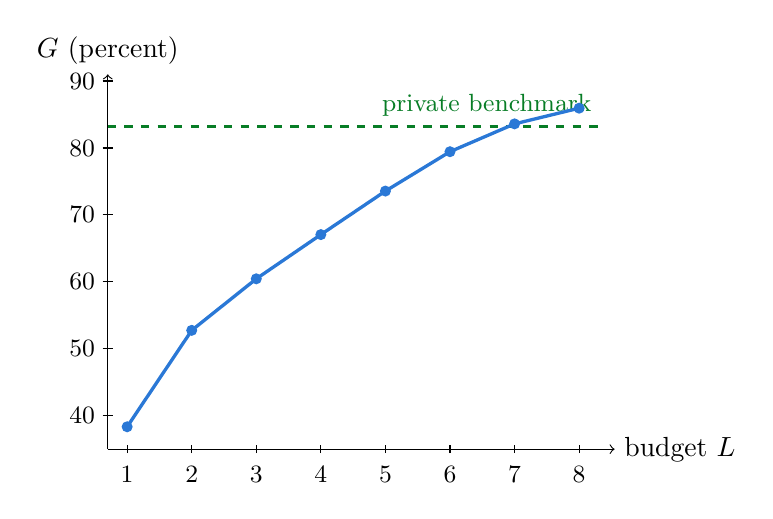
\begin{tikzpicture}[x=0.82cm,y=0.085cm]
\draw[->] (0.7,35) -- (8.55,35) node[right] {budget $L$};
\draw[->] (0.7,35) -- (0.7,91) node[above] {$G$ (percent)};
\foreach \x in {1,...,8} {\draw (\x,34.4)--(\x,35.6) node[below=4pt] {\small \x};}
\foreach \y in {40,50,...,90} {\draw (0.62,\y)--(0.78,\y) node[left=3pt] {\small \y};}
\draw[dashed,private,thick] (0.7,83.222784) -- (8.35,83.222784) node[above left] {\small private benchmark};
\draw[planner,very thick] plot coordinates {(1,38.346871) (2,52.753226) (3,60.452780) (4,67.058074) (5,73.560421) (6,79.443531) (7,83.601040) (8,85.942125)};
\fill[planner] (1,38.346871) circle (2pt);
\fill[planner] (2,52.753226) circle (2pt);
\fill[planner] (3,60.452780) circle (2pt);
\fill[planner] (4,67.058074) circle (2pt);
\fill[planner] (5,73.560421) circle (2pt);
\fill[planner] (6,79.443531) circle (2pt);
\fill[planner] (7,83.601040) circle (2pt);
\fill[planner] (8,85.942125) circle (2pt);
\end{tikzpicture}
\caption{Pooled-information discovery frontier by coordinated action budget. The first budget that weakly exceeds private clue-following is seven (DD-C-0008).}
\label{fig:frontier}
\end{figure}


Recovery budgets turn a performance gap into a resource diagnostic. They are still model-relative: a budget may count actions, money, time, robots, trials, or an admissible resource vector. In sequential settings, a fixed ex-ante budget and an expected stopping budget need not agree.

\section{Information, assignment, and incentives}
\label{sec:institutions}
% Claims: DD-C-0004, DD-C-0006, DD-C-0007, DD-C-0012, DD-C-0013
The benchmark protocols occupy three cells of an institutional matrix:
\begin{center}
\begin{tabular}{lll}
\toprule
Evidence / authority & Autonomous or unassigned & Coordinated or assigned\\
\midrule
Local/private evidence & Private clue-following & Private-team frontier\\
Pooled/shared evidence & Consensus or market & Planner portfolio\\
\bottomrule
\end{tabular}
\end{center}
The missing private-team cell allows agents to coordinate role-dependent policies before observing private signals, then act without communication. It isolates assignment capacity without granting pooled evidence at action time. This is a classical team-decision object in the sense of \citet{MarschakRadner1972}; DD-001 is a finite discovery specialization, not the invention of decentralized common-payoff policy design.

Let $T_N(E)$ be the best discovery probability attainable by ex-ante role policies under private evidence process $E$. Direct clue-following is feasible, so its value cannot exceed $T_N(E)$. A pooled planner can emulate any private team if it observes all private signals and retains the same or greater assignment authority, so under that emulation condition $T_N(E)$ cannot exceed the pooled frontier. These inequalities require a careful policy definition and are verified in DD-001 rather than assumed here.

Strategic autonomy adds a third margin. A reward rule maps outcomes into private utilities, and equilibrium may fail to maximize discovery even with a common posterior. Coverage games and valid-utility systems provide established ways to study this loss \citep{Vetta2002,Gairing2009}. The upstream equal-split game has a tight mixed discovery price-of-anarchy bound $2-1/N$, while a sole-rescue reward implements the top-$N$ portfolio in every pure equilibrium under stated assumptions \citep{Nakajima2026SharedDiscovery}. These are scoped results for one game and equilibrium class, not universal properties of discovery systems.

The design problem is therefore layered: choose what information is shared, what assignments are feasible, how rewards shape autonomous choice, and which equilibrium or learning outcome is selected. A mechanism that disperses actions by hiding useful evidence may be second-best to one that preserves information and rewards marginal coverage, but privacy, communication cost, incentive compatibility, or robustness can reverse that comparison.

\section{Correlated channels}
% Claims: DD-C-0009, DD-C-0010, DD-C-0014, DD-C-0015
Nominal report count is not evidence diversity. Agents may share data, retrieval sources, models, memories, or institutional incentives. Dependence can compress discovery before an explicit consensus rule is applied, while the same visible agreement may arise from very different provenance networks.

The upstream common-cue process is a tractable illustration. Some agents copy one latent cue while others draw independent signals. Its model-specific effective-channel count is
\[
N_{\mathrm{eff}}=N-K+\mathbf 1\{K\ge1\},
\]
where $K$ is the number of copiers. This counts independent generative draws in that process. It is not a general effective sample size, matrix rank, entropy, or channel capacity. The reported market/private crossover near copying probability $0.78846$ is a canonical computational result, not a general single-crossing theorem \citep{Nakajima2026SharedDiscovery}.

DD-003 replaces the scalar copying rate with latent source graphs. Pairwise correlation alone may be insufficient: two source structures can share correlations while differing in higher-order dependence, conditional independence, and the action portfolios they induce. Useful diagnostics may involve provenance overlap, source concentration, spectral quantities, conditional mutual information, or task-specific effective rank, but no universal choice is adopted here.

Dependence also changes the value of pooling. More reports may add little posterior information, while assignment still helps by preventing duplicate actions. Conversely, shared sources can be valuable when they reduce noise or coordinate complementary tests. The framework asks which link changes; it does not label correlation itself as harmful.

\section{Research agenda}
% Claims: DD-C-0001, DD-C-0017
The atomic benchmark supplies a reference point, not a completed general theory. The registered program consists of seven questions.

\begin{enumerate}
\item \textbf{Private-information teams (DD-001).} Characterize ex-ante role policies without action-time communication. Determine when clue-following, territorial specialization, or hybrid signal codebooks are optimal or merely feasible lower bounds.
\item \textbf{Information design (DD-002).} Ask whether Blackwell-more-informative public disclosure can concentrate equilibrium search under a fixed protocol. Begin from persuasion and informational Braess results rather than claiming harmful information is unprecedented.
\item \textbf{Source networks (DD-003).} Replace the common cue with latent provenance graphs and test which structural diagnostics predict discovery beyond nominal reports or pairwise correlation.
\item \textbf{Sequential discovery (DD-004).} Introduce outcome feedback, stopping, and parallel-versus-adaptive capacity. Approximation claims require adaptive submodularity or another stated structure \citep{GolovinKrause2011}.
\item \textbf{Overlapping coverage (DD-005).} Move from atomic modular value to set-valued, multi-target, or submodular coverage. Greedy guarantees require the hypotheses of established submodular results \citep{NemhauserEtAl1978}.
\item \textbf{Discovery mechanisms (DD-006).} Jointly design reporting, action differentiation, and credit under private information, budget balance, collusion, and observability constraints.
\item \textbf{Empirical audits (DD-007).} Determine which data identify or bound protocol loss, recovery budgets, action concentration, source concentration, effective channels, and latent copying.
\end{enumerate}

Each direction has a separate feasibility class, objective, identification problem, and evidence status. Computation can establish finite-instance values or refute conjectures but does not turn a pattern into a theorem. The claim ledger therefore distinguishes sourced upstream results, derived identities, independent reproductions, checked computations, observations, conjectures, and open questions.

\section{Measurement and applications}
% Claims: DD-C-0001, DD-C-0011
An empirical discovery audit begins with an event ontology. What is the candidate space? What constitutes evidence, an action, coverage, and success? Which actors share sources, models, or instructions? Which actions are simultaneous, sequential, or contingent on failure? Without those choices, ``duplication'' and ``diversity'' are labels rather than estimands.

At minimum, an audit can report action concentration, unique-action counts, overlap under a declared coverage function, provenance concentration, and outcome coverage. Estimating a frontier or protocol loss is harder: it requires a posterior or score model, a feasible counterfactual protocol class, and assumptions supporting off-policy evaluation or structural extrapolation. Recovery budgets inherit the same counterfactual burden. Descriptive concentration can diagnose compression without identifying its welfare cost.

\subsection*{A staged audit design}
A practical audit can proceed in six stages. First, define the unit of a candidate and action. A paper topic, compound, market, tool call, or answer string may require a taxonomy before duplicates can be recognized. Second, reconstruct timing: which evidence and prior actions were observable when each choice was made? Third, attach provenance at the narrowest defensible level---dataset, source, model, retrieval result, laboratory, or shared instruction---without equating missing provenance with independence.

Fourth, estimate descriptive portfolio quantities with uncertainty: unique actions, concentration, pairwise and higher-order overlap, covered candidate mass, and success. The estimator should handle censoring, ambiguous matches, and repeated actions that intentionally replicate. Fifth, specify one or more feasible counterfactual protocols. A top-score reallocation is not feasible if expertise or capacity prevents reassignment; a private-information counterfactual is not recoverable after only pooled summaries were logged. Sixth, conduct sensitivity analysis over posterior calibration, coverage definitions, action costs, and latent dependence. A point estimate of protocol loss without these choices can be more misleading than a transparent descriptive audit.

Identification differs by diagnostic. Action concentration is observed once actions are encoded, though sampling and matching error remain. Source concentration requires a definition of source and a model for missing provenance. Protocol loss requires both an attainable frontier and the expected value of the implemented rule. A recovery budget additionally extrapolates performance across capacities. Latent copying may be partially disciplined by duplication and shared failures, but similar patterns can arise from common rational response to strong evidence. DD-007 therefore begins with synthetic recovery tests before interpreting observational estimates.

Reporting should preserve this ladder. A dashboard may safely display counts and overlaps as observations, present model-based frontier estimates with assumptions, and reserve causal language for designs that justify it. The aim is not to make every organization estimate a structural model; it is to prevent a concentration chart from silently becoming a welfare claim.

In science, evidence is prior research and actions are experiments; coverage concerns hypotheses, mechanisms, or empirical regions distinguishable by those experiments. Replication means repeated action may be socially valuable, so robustness and credibility enter $v$. In R\&D, evidence is technical and market learning, actions are prototypes or development paths, and budgets include capital, personnel, and technical dependencies. In venture portfolios, actions are investments and coverage represents distinct market or technology hypotheses; payoff is heavy-tailed and non-binary, so the box model is only a reference.

For multi-agent AI, evidence includes prompts, retrieval, tools, model weights, memory, and evaluator feedback. Actions may be proposed answers, investigations, code changes, or tool calls. Nominal agent count is a poor proxy for evidence diversity when sources and model state are shared. Posterior sampling, role differentiation, diverse retrieval, marginal-coverage rewards, and explicit provenance are candidate interventions, not validated universal remedies.

Scientific communities already face dynamic experiment-choice, career, and knowledge-network effects far richer than the atomic benchmark \citep{RzhetskyEtAl2015,March1991,Kitcher1990,Zollman2007}. The framework's role is to make comparison dimensions explicit so richer models do not attribute an information effect to a simultaneous change in action allocation.

\section{Limitations}
% Claims: DD-C-0017
The framework has six immediate limitations. First, its central decomposition is accounting; explanatory and prescriptive force comes only from characterizing a frontier or loss. Second, a frontier depends on institutional authority and may be unobservable or computationally intractable. Third, the atomic top-$L$ rule and redundant-hit identity do not transfer automatically to overlapping or sequential value. Fourth, reward and equilibrium models require behavioral assumptions that common-objective notation suppresses. Fifth, provenance and effective channels are often latent, so descriptive action diversity does not identify information diversity. Sixth, no terminology review can establish broad novelty; ``distributed discovery,'' ``information frontier,'' ``protocol loss,'' and ``effective channels'' all have neighboring uses.

The canonical computations are exact or high precision only within their declared finite model. The anonymous-market equilibrium value and copying crossover have not received independent local implementations. Application mappings are hypotheses about primitives, not empirical validation. Communication budgets remain outside DD-001 until the zero-communication policy class is stable.

These limits are productive. They specify what a claim must include: world and evidence model, information access, action technology, protocol class, budget, timing, objective, reward rule, source or run, and evidence status. A compact benchmark can then serve as a comparison point without claiming to explain every discovery institution.

\section{Conclusion}
% Claims: DD-C-0001, DD-C-0002
Distributed discovery separates forming beliefs from allocating attempts. The information frontier asks what discovery is attainable from available evidence under declared authority and constraints. Protocol loss asks how much of that attainable value an implemented rule destroys. The distinction reveals why a better ranking need not yield a better search and why more agents need not mean more effective channels.

The Shared Discovery Paradox supplies the atomic case: one target, noisy clues, and a portfolio compressed by a one-answer rule. The broader agenda begins when private evidence, strategic incentives, source networks, sequential feedback, and overlapping coverage are made explicit. Its discipline is modest but useful: hold margins fixed when making comparisons, preserve evidence status, and treat open cells as questions rather than conclusions.

\bibliographystyle{plainnat}
\bibliography{generated/references}
\end{document}
